\begin{frame}{重积分的计算}
	\linespread{1.2}
	\begin{enumerate}
	  \item 二重积分在极坐标下的定限
	  \item 三重积分的定限(何时使用“1+2”)
	  \item 对称性在重积分计算中的应用
	  \item 三重积分在柱坐标下的定限
	  \item 三重积分在球坐标下的定限
	  \item 各种定限方法的抽象描述
	  \item 一般变换下重积分的计算(Jacobi行列式)
	\end{enumerate}
\end{frame}

\begin{frame}
	\linespread{1.5}
% 	$\star$
	\ba{1、}设$D$由$y=x^3,y=1,x=-1$所围成,则
	$\ds\iint_Dx[1+yf(x^2+y^2)]\d\sigma=$
	\underline{\uncover<2->{\;\b{$-\df52$}}\;}.\\[1em]
	
% 	\pause\pause
	\ba{2、}设$D$由$x^2+y^2\leq x+y$确定,则
	$\ds\iint_D(x+y)\d\sigma=$
	\underline{\uncover<3->{\;\b{$\df{\pi}2$}}\;}.\\[1em]
	
% 	\pause\pause
	\ba{3、}设$D$由$x=-2,y=0,y=2$和$x=-\sqrt{2y-y^2}$所围,则
	$\ds\iint_Dy\d\sigma=$
	\underline{\uncover<4->{\;\b{$4-\df{\pi}2$}}\;}.\\[1em]
	
% 	\pause\pause
	\ba{4、}$\ds\iint_{\mathbb{R}^2}\min\{x,y\}e^{-x^2-y^2}\d\sigma=$
	\underline{\uncover<5->{\;\b{$-\sqrt{\df{\pi}2}$}}\;}.
\end{frame}

\begin{frame}
	\linespread{1.5}
	\it
	\begin{exampleblock}{对称性在二重积分中的应用}
		设区域$D$关于$x=0$对称,则
		\begin{enumerate}
		  \item 若$f(x,y)$关于$x$为奇函数,则
		  $$\ds\iint_Df(x,y)\d\sigma=0$$
		  \item \pause 若$f(x,y)$关于$x$为偶函数,则
		  $$\ds\iint_{D}f(x,y)\d\sigma=2\ds\iint_{D_1}f(x,y)\d\sigma,$$
		  其中$D_1$为$D$中$x\geq0$的部分
		\end{enumerate}
	\end{exampleblock}
\end{frame}

\begin{frame}
	\linespread{1.5}
	\it
	\begin{block}{推论}
		设区域$D$关于$x=a$对称,则
		\begin{enumerate}
		  \item 若$f(x,y)$关于$x=a$反对称{\b $(f(x,y)=-f(2a-x,$
		  $y))$},则
		  $$\ds\iint_Df(x,y)\d\sigma=0$$
		  \item \pause 若$f(x,y)$关于$x=a$对称{\b $(f(x,y)=f(2a-x,y))$},则
		  $$\ds\iint_{D}f(x,y)\d\sigma=2\ds\iint_{D_1}f(x,y)\d\sigma,$$
		  其中$D_1$为$D$中$x\geq a$的部分
		\end{enumerate}
	\end{block}
\end{frame}

\begin{frame}
	\linespread{1.5}
	\it
	\begin{exampleblock}{对称性在三重积分中的应用}
		设区域$\Omega$关于$x=0$对称,则
		\begin{enumerate}
		  \item 若$f(x,y,z)$关于$x$为奇函数,则
		  $$\ds\iiint_{\Omega}f(x,y,z)\d V=0$$
		  \item \pause 若$f(x,y,z)$关于$x$为偶函数,则
		  $$\ds\iiint_{\Omega}f(x,y,z)\d V
		  =2\ds\iiint_{\Omega_1}f(x,y,z)\d V,$$
		  其中$\Omega_1$为$\Omega$中$x\geq0$的部分
		\end{enumerate}
	\end{exampleblock}
\end{frame}

\begin{frame}
	\linespread{1.5}
	\begin{exampleblock}{二重积分的轮换对称性}
		{\it 设区域$D$关于$y=x$对称,则}
		$$\ds\iint_Df(x,y)\d\sigma=\ds\iint_Df(y,x)\d\sigma$$
	\end{exampleblock}
	\bigskip\pause
	\ba{例:}设$D:(x-2)^2+(y-2)^2\leq 1$,则
	$$\ds\iint_D\df{3x^3-2y^3}{x^3+y^3}\d\sigma=\pi$$
	\bigskip\pause
	\ba{例:}$\dint_0^1f(x)\d x=A$,则
	$\dint_0^1\dint_x^1f(x)f(y)\d y\d x=\df{A^2}2$
\end{frame}

\begin{frame}
	\linespread{1.2}
	\ba{思考:}
		证明:
		$$\dint_0^t\d t_1\dint_0^{t_1}\d t_2\ldots
		\dint_0^{t_{n-1}}\prod\limits_{i=1}^nf(t_i)\d t_n
		=\df1{n!}{\left[\dint_0^tf(s)\d s\right]^n}$$
	\bigskip\pause
	\alert{提示:}{\it\b $I_2(t)=\df12\left[\dint_0^tf(s)\d s\right]^2$,
	$$I_n(t)=\dint_0^tf(t_1)I_{n-1}(t_1)\d t_1$$
	利用数学归纳法证明
	}
\end{frame}

\begin{frame}
	\linespread{1.5}
	\ba{例:}设$D$为$x^2+y^2\leq 4$在第一象限中的部分,$f(x)$连续且
	恒大于零,则$\ds\iint_D\df{a\sqrt{f(x)}+b\sqrt{f(y)}}
	{\sqrt{f(x)}+\sqrt{f(y)}}\d\sigma=$
	(\underline{\uncover<2->{\;\b{D}}\;})
	\begin{enumerate}[(A)]
	  \item $ab\pi$
	  \item $\df{ab}2\pi$
	  \item $(a+b)\pi$
	  \item $\df{a+b}2\pi$
	\end{enumerate}
\end{frame}

\begin{frame}
	\linespread{1.5}
	\ba{例:}计算三重积分$I=\ds\iiint_{\Omega}(x+y)\d V$,其中$\Omega$由
	$x=0,x=1,x^2+1=\df{y^2}{b^2}+\df{z^2}{c^2}$所围成。
	
	\pause\alert{提示:}{\it\b 根据对称性
	$$\ds\iiint_{\Omega}y\d V=0,$$
	剩余的部分采用“$1+2$”的方式计算.
	}
\end{frame}

\begin{frame}
	\linespread{1.5}
	\begin{block}{推论}
		{\it 设区域$D$关于$y=x$对称,且$f(x,y)=-f(y,x)$,则}
		$$\ds\iint_Df(x,y)\d\sigma=0$$
	\end{block}
	\bigskip\pause
	\ba{例:}设$D:x^4+y^4\leq 1$,则
	$$\ds\iint_D\df{x^2-y^2}{x^2+y^2+1}\d\sigma=0$$
\end{frame}

\begin{frame}
	\linespread{1.5}
	\begin{exampleblock}{三重积分中的轮换对称性}
		{\it 设区域$\Omega$中$x,y,z$对位对等{\b $(x,y,z$任意交换$\Omega$不发生改变$)$},则
		在积分$\ds\iiint_{\Omega}f(x,y,z)\d V$中$x,y,z$任意交换不改变
		积分的值。}
	\end{exampleblock}
	\bigskip\pause
	\ba{例:}设$\Omega:\df{x^2}{a^2}+\df{y^2}{b^2}+\df{z^2}{c^2}\leq 1$,
	则
	$$\ds\iiint_{\Omega}(x+y+z)^2\d V=\df{4}{15}\pi abc(a^2+b^2+c^2)$$
\end{frame}


\begin{frame}
	\linespread{1.5}
	\ba{例:}设$f(x)$连续,$F(t)=\dint_1^t\dint_y^tf(x)\d x\d y$,则
	$F'(2)=$
	(\underline{\uncover<2->{\;\b{B}}\;})
	\begin{enumerate}[(A)]
	  \item $2f(2)$
	  \item $f(2)$
	  \item $-f(2)$
	  \item $0$
	\end{enumerate}
	
	\pause\alert{提示:}{\it\b  
	$F(t)=\dint_1^t\dint_1^xf(x)\d y\d x=\dint_1^t(x-1)f(x)\d x$
	}
\end{frame}

\begin{frame}
	\linespread{2}
	\ba{例:}设$f(x,y)$在$D:0\leq x\leq 1,0\leq y\leq 1$上连续,
	$f(0,0)=-1$,求
	$$\limx{0^+}\df{\dint_0^{x^2}\dint_x^{\sqrt t}f(t,u)\d u\d t}
	{1-e^{-x^3}}$$
	
	\pause\alert{提示:}{\it\b $\df13$,使用L' Hospital法则结合积分中值定理。
	}
\end{frame}

\begin{frame}
	\linespread{2}
	\ba{例:}设$f(x,y)$在单位圆内一阶偏导函数连续,且在边界上函数值均为零,
	$D:\e^2\leq x^2+y^2\leq 1$,证明:
	$$f(0,0)=\lim\limits_{\e\to0^+}\df{-1}{2\pi}
	\ds\iint_D\df{xf'_x+yf'_y}{x^2+y^2}\d\sigma$$
	
	\pause\alert{提示:}{\it\b 将原积分换成极坐标下的形式,结合积分中值定理
	}
\end{frame}

\begin{frame}
	\linespread{2}
	\ba{例:}设$f(x)$在区间$[a,b]$连续且恒大于零,证明:
		$$\dint_a^bf(x)\d x\dint_a^b\df{\d x}{f(x)}\geq (b-a)^2$$
	
	\pause\alert{提示:}{\it\b Cauchy-Schwartz不等式
	$$\left(\dint_a^bf(x)g(x)\d x\right)^2
	\leq\dint_a^bf^2(x)\d x\cdot\dint_a^bg^2(x)\d x$$
	}
\end{frame}

\begin{frame}
	\linespread{2}
	\ba{例:}按先$y$后$z$后$x$的积分次序重写以下累次积分
	$$\dint_0^1\dint_0^x\dint_0^{xy}f(x,y,z)\d z\d y\d x$$
	\begin{center}
		\pause \resizebox{!}{5cm}{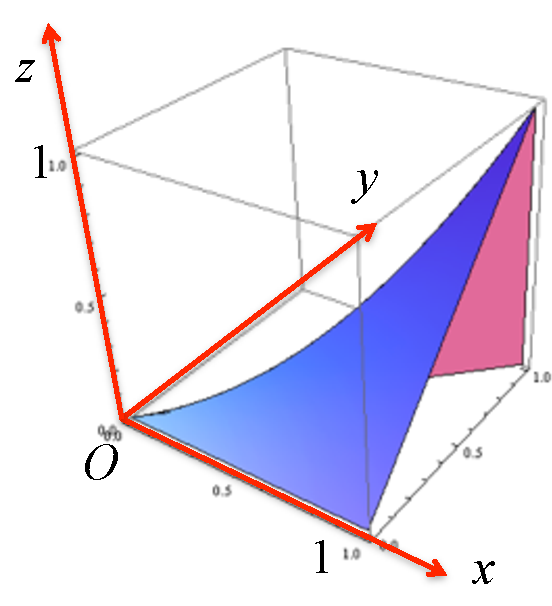
\includegraphics{./images/ch11/xyzC.pdf}}
	\end{center}
\end{frame}

% \begin{frame}
% 	\small
% 	1、交换积分次序
% 	 \begin{itemize}
% 	    \item $\dint_0^2\dint_{x^2}^xf(x,y)\d y\d x$
% 	    \item $\dint_{-\pi/4}^{\pi/2}\dint_0^{2a\cos\theta}
% 	    f(\rho\cos\theta,\rho\sin\theta)\rho\d\rho\d\theta$
% 	 \end{itemize}
% 	2、设$f(x)$在$[a,b]$上单调递增且恒为正,证明
% 		$${\dint_0^1xf\,^2(x)\d x}{\dint_0^1f(x)\d x}\leq
% 		{\dint_0^1f\,^2(x)\d x}{\dint_0^1xf(x)\d x}$$
%    	3、计算极限
% 		$\lim\limits_{n\to\infty}\df 1{n^4}\iiint_{r\leq n}[r]\d V,$
% 		其中$r=\sqrt{x^2+y^2+z^2}$
% 		
% 	4、$f(t)$连续,$F(t)=\ds\iiint_{\Omega}[z^2+f(x^2+y^2)]\d V$,其中
% 		$\Omega$由$x^2+y^2\leq t^2,0\leq z\leq h$确定,求$F'(t)$和
% 		$\lim\limits_{t\to 0^+}\df{F(t)}{t^2}$
% \end{frame}

\begin{frame}{$n$重积分*}
	\linespread{1.2}
	\ba{例:}求$n$维单纯形
		$$T_n(a):\; x_i\geq 0\,(i=1,2,\ldots,n),\;
		\sum\limits_{i=1}^nx_i\leq a$$
		的体积$(a>0)$。
		
	\bigskip\pause
	\alert{提示:}{\it\b 
	$$V(T_n(a))=\dint_0^aV(T_{n-1}(a-x))\d x
% 	=\dint_0^a\df{(a-x)^{n-1}}{(n-1)!}\d x
	={\df{a^n}{n!}}$$}
\end{frame}



\begin{frame}
	\linespread{1.2}
	\ba{例:}
		求$n$维单位球
		$$S_n:\sum\limits_{k=1}^nx_k^2\leq 1$$
		的体积。
		
	\bigskip\pause
	\alert{提示:}{\it\b
	$${\Gamma(\alpha)=\dint_0^{+\infty}x^{\alpha-1}e^{-x}dx,\;(\alpha>0)}$$
	\pause
	$${V_n=\df{2\pi^{n/2}}{n\Gamma(n/2)}}\to 0\quad(n\to\infty)$$}
\end{frame}
